\documentclass[yellow]{beamer}
\usepackage{beamerthemesplit}
\usepackage{amsmath,graphicx,amssymb,amsfonts,pgfarrows,pgfnodes,amssymb,amsfonts}
\usepackage{hyperref}
\usepackage{graphicx}
\hypersetup{pdfpagemode=FullScreen} 
\usetheme{Warsaw}
\useinnertheme{circles}
\useinnertheme{rounded}
\useoutertheme[subsection=false]{smoothbars}
\usecolortheme{sidebartab}


\title{Why the Arduino is Here to Stay}
\author{Thomas Swartz}
\institute{The University of Scranton}
\date{\today}


\begin{document}

\frame{\titlepage}


\section{The Arduino}

\begin{frame}
\frametitle{What exactly is the Arduino?}
\begin{center}
	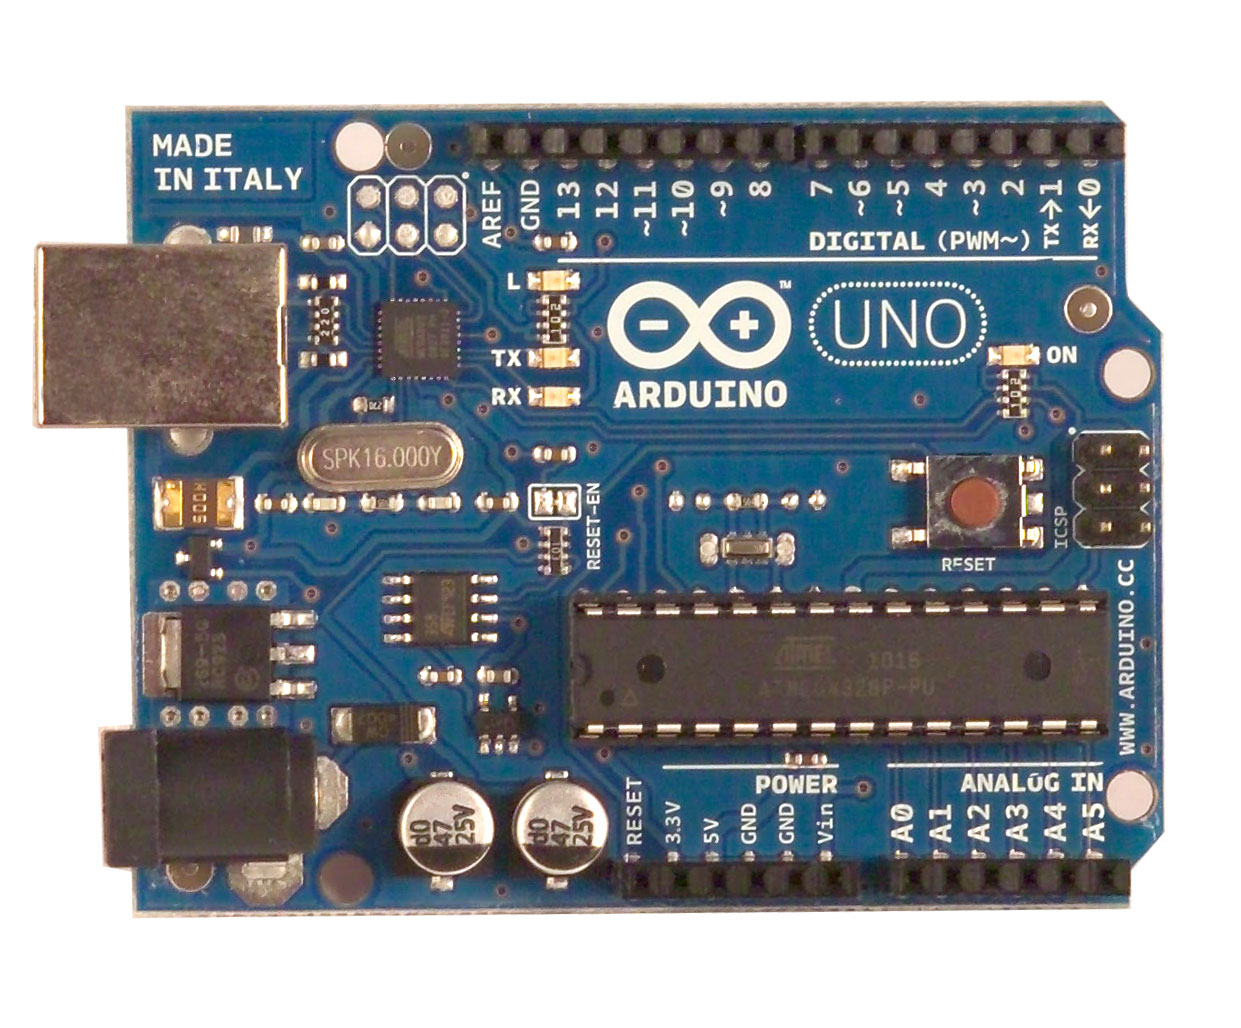
\includegraphics[width=0.50\textwidth]{arduinounofront.jpg}
\end{center}
Arduino is an open-source electronics prototyping platform based on flexible, easy-to-use hardware and software.\\ 
It's intended for artists, designers, hobbyists, and anyone interested in creating interactive objects or environments.
\end{frame}

\begin{frame}
\frametitle{What exactly is the Arduino?}
There are over 100,000 Arduinos sold \pause in the past 3 years.\\ 
\pause
As of 2/2/2011, there are 50,000 derivatives and shields made for the Arduino. \\
\pause
That makes for a total of 150,000 Arduinos (and 150,000 projects) in 3 years
\end{frame}

\begin{frame}
\frametitle{What exactly is the Arduino?}
\begin{itemize}
	\item<1-> Arduino can sense the environment by receiving input from a variety of sensors and can affect its surroundings by controlling lights, motors, and other actuators.
	\item<2-> The microcontroller on the board is programmed using the Arduino programming language (based on Wiring) and the Arduino development environment (based on Processing).
	\item<3-> Arduino projects can be stand-alone or they can communicate with software on running on a computer (e.g. Flash, Processing, MaxMSP).
\end{itemize}
\end{frame}

\begin{frame}
\frametitle{What exactly is the Arduino?}
\begin{itemize}
	\item<1-> The boards can be built by hand or purchased preassembled 
	\item<2-> The software can be downloaded for free
	\item<3-> The hardware reference designs (CAD files) are available under an open-source licenses
\end{itemize}
\end{frame}

\section{What Can You Do With It?}

\begin{frame}
\frametitle{What can you do with an Arduino?}
\begin{center}
\pause 
\emph{\huge{ANYTHING}}

\end{center}
\end{frame}

\begin{frame}
\frametitle{A Coffee Pot That Tweets When It's Done}
\begin{center}
	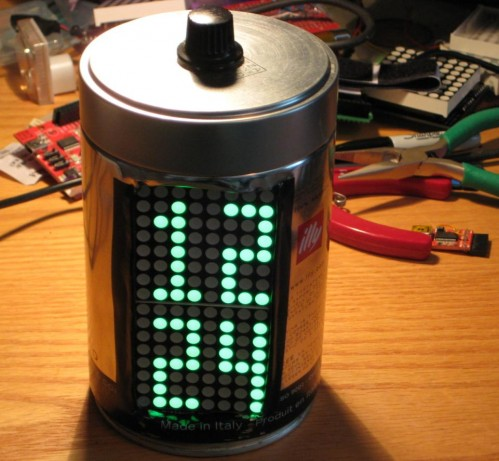
\includegraphics[width=0.75\textwidth]{coffee.jpg}
\end{center}
\end{frame}

\begin{frame}
\frametitle{A Jeopardy Game Using Staples Easy Buttons}
\begin{center}
	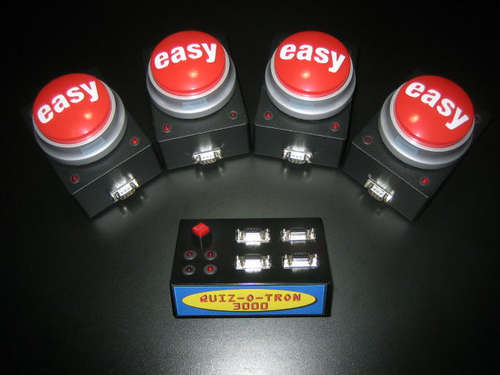
\includegraphics[width=0.75\textwidth]{jeopardy.jpg}
\end{center}
\end{frame}

\begin{frame}
\frametitle{A Portal Gun}
\begin{center}
	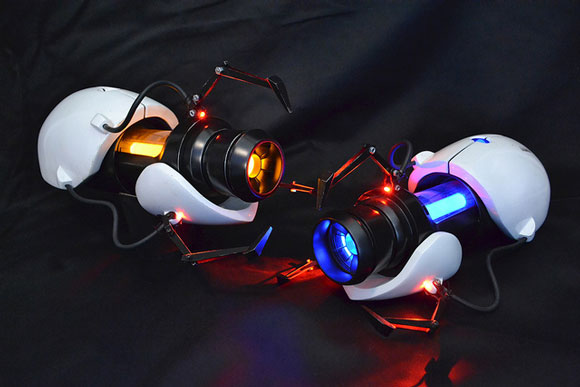
\includegraphics[width=0.75\textwidth]{portal.jpg}
\end{center}
\end{frame}

\begin{frame}
\frametitle{A Metroid Gun}
\begin{center}
	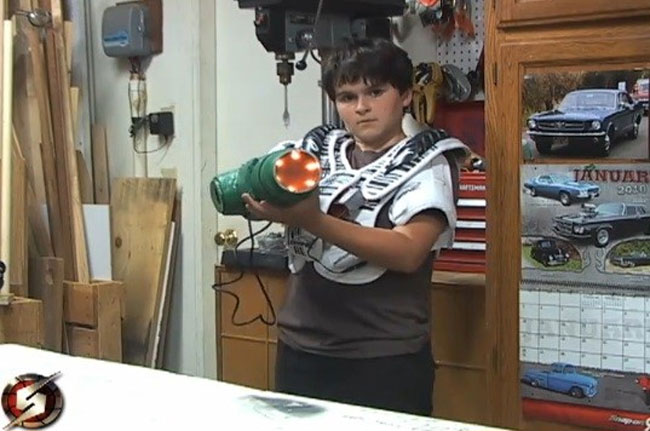
\includegraphics[width=0.75\textwidth]{samus.jpg}
\end{center}
\end{frame}

\begin{frame}
\frametitle{A (Sexy) Tron Costume}
\begin{center}
	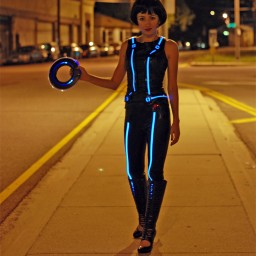
\includegraphics[scale=0.75]{tron.jpg}
\end{center}
\end{frame}

\begin{frame}
\frametitle{A Wearable Turn Signal for Biking}
\begin{center}
	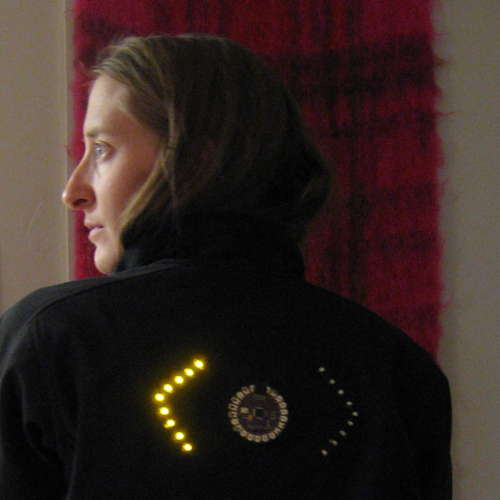
\includegraphics[width=0.5\textwidth]{bike.jpg}
\end{center}
\end{frame}

\begin{frame}
\frametitle{A Simple Robot}
\begin{center}
	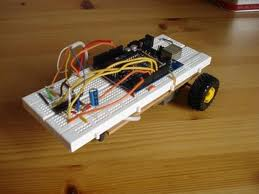
\includegraphics[width=0.5\textwidth]{images-2.jpeg}
\end{center}
\end{frame}

\begin{frame}
\frametitle{An Even Better Robot}
\begin{center}
	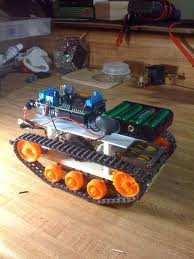
\includegraphics[width=0.5\textwidth]{images-1.jpeg}
\end{center}
\end{frame}

\begin{frame}
\frametitle{A Word Clock}
\begin{center}
	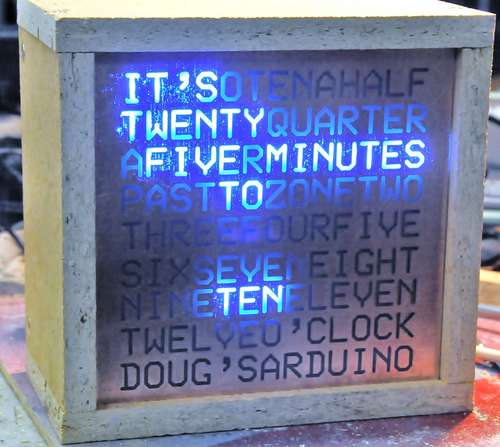
\includegraphics[width=0.5\textwidth]{wordclock.jpg}
\end{center}
\end{frame}

\section{So Why is it Successful?}

\begin{frame}
\begin{center}\huge So Why is it So Successful?
\end{center}
\end{frame}

\begin{frame}
\frametitle{It Just Works}
\begin{itemize}
\item<1-> The IDE runs on Mac, Windows, and Linux
\item<2-> The drivers actually work on systems other than Windows
\item<3-> Libraries, Easy-to-do simple things, Easy-to-do hard things
\item<4-> Lightweight and doesn't need a computer to run
\item<5-> Sensors and Shields
\item<6-> Simple, but not TOO simple!
\item<7-> Low cost
\item<8-> Open Source
\end{itemize}
\end{frame}

\begin{frame}
\frametitle{There is So Much Support}
Anything you want to do is available to learn and create
\begin{center}
	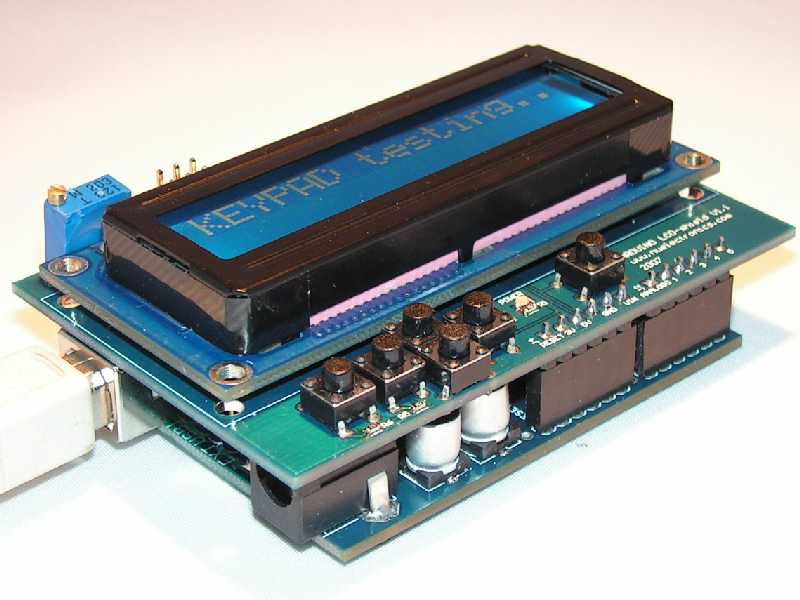
\includegraphics[width=0.5\textwidth]{lcd_shield_2.jpg}
\end{center}
\end{frame}

\section{How is it Better?}
\begin{frame}
\frametitle{How Does it Compare to What We Use Now?}
Lets Compare:\\
\begin{center}
\begin{tabular}{ l || c | c | c }
   & Arduino & C-Stamp  & Basic Stamp\\
  \hline
  Cost			& \$25 	& \$100	& \$50 \\
  Number of Pins	& 26 		& 20 		& 14 \\
  Voltage		& 1.5 -- 24 V 	& 3 -- 24 	& 3 -- 24 \\
  RAM			& 30 Kb		& 32 Kb 	& 32 Kb \\
  Programming Interface	& USB		& Serial 	& Serial \\
\end{tabular}
\end{center}
\end{frame}

\begin{frame}
\begin{center}\huge{Questions?}\end{center}
\end{frame}

\section{Show and Tell!}
\begin{frame}
\frametitle{Real Life Demo}
\begin{center}
\begin{itemize}
	\item RGB Color Mixer
	\item KITT
	\item Special Treat
\end{itemize}
\end{center}
\end{frame}
\end{document}
